\documentclass[twocolumn]{article}
\usepackage{authblk}
\usepackage{blindtext}
\usepackage{multicol}% http://ctan.org/pkg/multicols
\usepackage{graphicx}
\usepackage{subcaption}
\usepackage{cite}
\usepackage[table,xcdraw]{xcolor}
\newcommand{\FA}[1]{\begingroup\color{magenta}#1\endgroup}
\newcommand{\TODO}[1]{\begingroup\color{red}#1\endgroup}
%opening
\begin{document}



\title{\textit{MSF: Modulated Sub-path Finder} }

\author[1]{Mariam R Farman}
\author[1,2]{Fabian Amman}
\author[1]{Ivo L Hofacker}
\affil[1]{Institute for Theoretical Chemistry,Theoretical Biochemistry Group,University of Vienna,Austria}
\affil[2]{Department of Chromosome Biology, Max F. Perutz Laboratories,University of Vienna,Austria}



\maketitle

\begin{abstract}
Differentially expressed genes play an important role in giving
insights to a phenotype. These DEGs are then used to identify the
pathways altered during changing biological conditions. We developed a
novel approach to find the maximal significantly dis-regulated
sub-paths or cluster of genes from the cell signaling network, giving
these sub-paths an overall significance of modulation by combining the
individual p-values of the genes.
\end{abstract}

\section*{Keywords}

Differentially expressed genes, Pathway analysis, Combining \textit{p}-value, Cell signaling network, Modulated Sub-paths


\section*{Background}

High throughput sequencing techniques have been widely used to yield
the differentially expressed genes (DEG)~\cite{DEG}. To this end,
changes in transcript abundance is measured, e.g.~by next generation
sequencing techniques, and interpreted as an indicator of differential
expression of genes. Differentially expressed genes can be used to get
insights into the mechanism underlying differences conditions, such as
healthy versus diseased. In the first instance, the differential gene
expression analysis informs about the magnitude of expression changes
between the conditions which is the log fold change, a sign of the log fold change and the confidence level
of observing a authentic change, often expressed as
\textit{p}-value. These lists of differentially expressed genes are
then used to extract meaningful insights, for example the genes that
could be important for a particular condition or maybe the target gene
of any infection or disease. Out of all high throughput analysis
methods currently in use, pathway-based analysis has become an
important tool to further interpret the results of a DGEA and to
acquire understandings of the perturbations in a biological
system. Biological pathways are set of genes contained in a functional
unit. They help to identify pathways or networks that may be altered
during a change of condition providing important information about
diseases and its treatment process~\cite{Khatri2012}. Pathway-based
methods use the predefined pathways or networks such as
KEGG~\cite{Kegg} and Reactome~\cite{Reactome}, the expression
measurements of the genes obtained from differential gene expression
analysis (DGEA) in combination with statistical methods and algorithms to
identify specifically modulated pathways and processes~\cite{Campos}.

The existing pathway-based analysis approaches use different research
designs, which can be categorized into ORA (Over-representation
analysis), FCS (Functional class scoring) and pathway topology based
methods. ORA is the first and the most basic method of pathway
analysis. It uses a user defined cut-off for the log-fold change and
p-value from the DGEA (most commonly using absolute log-fold change
$\geq$ 2 and \textit{p}-value $\leq$ 0.05) to define a list of
differentially expressed genes. Subsequently, sets of genes associated
with annotated pathways are tested for being overrepresented in the
set of differentially expressed genes. To this end, hypergeometric
distribution, chi-square tests, binomial probability or the Fisher’s
exact test are used. Thereby the information of the topology of the
pathways are ignored~\cite{Bayer}. Futhermore, ORA assumes the
pathways are independent of each other and ignores the fact that
biological pathways cross-talk and overlap~\cite{Khatri2012,Campos}.

Unlike ORA, FCS has no artificial cut-off to define DEG list and does
not assume genes to be independent of each other. FCS works in three
step, first it calculates the gene-level statistics including correlation of molecular measurements, ANOVA, Q-statistic, signal-to-noise ratio, t-test and Z-score. In the second step the statistics of individual genes are transformed to a individual pathway-level statistic and finally the
pathway-level statistics are accessed. Although FCs covers some of the
limitations from ORA, it still lacks the topology, cross-talk and
overlap of the pathways~\cite{Khatri2012,Campos}. Pathway topology
based methods are similar to FCS except that they consider the
topology of each gene during the gene-level
statistics but still are unable to consider a link between different pathways~\cite{Khatri2012}.

On these grounds we propose a novel approach to make use of the rich
pathway annotation resources available to gain additional functional
insights from basic DGEA. To this, we
start with the presupposition that expression of neighboring genes
within a functional pathway are not independent from each
other. Rather, they are often regulating each others expression or are
part of the same regulon~\cite{Michalak}. Second, we
understand that the categorization of links between genes into labeled
pathways is often an arbitrary one, given the extensive cross talk
between different pathways. Although this categories have proven to be
useful in many situations, they force a certain perspective onto the
interpretation of novel data. Based on this two principles, we aim to
find sub-modules within predefined networks which exhibits as a whole
significant differential expression changes. As input information on
functional links between genes, provided by e.g. KEGG or Reactome, and
information on the differential expression status of single genes,
resulting from a DGEA, are required. As a result the analysis returns
sub-modules and their joint confidence scores, reflecting how the
perturbation is migrated through the network. Furthermore, the entry
points of perturbation in the networks and overlap with conventional
pathway categories are returned. All of this can be helpful to
understand cause end effect of a stimulus and might inform about
potential points of intervention. The proposed algorithm was
implemented as a java program, which was named Modulated SubPath
Finder (\texttt{MSF}).

\section*{Methods}
\texttt{MSF} is developed as a novel heuristic approach in Java to
find the modulated sub-paths of gene interactions from the cell
signaling network. The network has nodes corresponding to genes and
edges representing their relationship. The pipeline of identification
of modulated sub-paths from a network by \texttt{MSF} is depicted in
Fig (1).

\texttt{MSF} uses the individual gene's \textit{p}-values generated
from the DGEA. The \textit{p}-value
expresses the probability that the hypothesis of unmodified gene
expression can be rejected for a given statistical model. To find
significantly modulated sub-paths individual \textit{p}-values of the
vicinal genes in the global network are combined into a single
combined \textit{p}-value, using a statistical method for combining
dependent \textit{p}-values described by~\cite{Hartung}. Using the
inverse normal method, individual gene \textit{p}-values $p_i$ are
first transformed to its corresponding normal score $t_i$,

\[ t_i = \Phi^{-1}(p_i) \]  

Then using these normal scores, the correlation \textit{Co} between genes are calculated, 

\[ Co (t_i, t_j) =\varrho \]

followed by correction of the correlation \textbf{k}. The normal
scores, correlations and the correction of correlation are applied to
the inverse normal function to calculate the individual
\textit{p}-value for a sub-path \textit{Cp}. \newline

$  {\scriptstyle Cp(\varrho,K) = \frac{\sum_{i=1}^{n} \lambda_i t_i}{\sqrt{\sum_{i=1}^{n} \lambda_i^2 +[(\sum_{i=1}^{n} \lambda_i)^2- \sum_{i=1}^{n} \lambda_i^2]\{\varrho+k\cdot\sqrt{\frac{2}{n+1}} (1-\varrho)}}} $\\ \newline

Lambda $\lambda$ are the weights for each gene, For the moment equal
weights are given to all genes and \textbf{k} used is 0.2 as used by authors. An
overall \textit{p}-value of a sub-path will express the significance
of all genes in the sub-path being modulated together.

To reduce the complexity to score all possible connected sub-modules
\texttt{MSF} applies a three steps heuristic as described in the
following.\newline
 
\subsection*{Overview of our method}

\textbf{Initial Modulated Sub-paths}

\texttt{MSF} constructs the first sub-path starting with the genes
associated with the lowest (most significant) \textit{p}-value from
the network. It tries to extend the
sub-path to the most significant neighboring gene. A single combined
\textit{p}-value is calculated for the two genes. If the combined
\textit{p}-value is smaller than the minimal individual gene's
\textit{p}-values, the extended sub-path is accepted. Then the next most significant neighboring gene is added to the sub-path and the combined \textit{p}-value is calculated, if the new combined p-value of three genes is smaller than the combined p-value of the first two genes,the extended sub-path is accepted. This step is iteratively repeated until no further extension is accepted. In this
case the process starts over with all remaining genes not yet in a
significant modulated sub-path. This step identifies all the trivial
sub-paths that are modulated in the whole network~(Fig.~1b).\newline

\textbf{Extending Modulated Sub-paths}

In the next step the initial modulated sub-paths are used to check if
they could further be extended beyond the immediate neighborhood.
This is done by testing all possible extension up to N genes for
all genes in the sub-path. Again, this step is iteratively repeated until no
further genes are added to the significant differentially expressed
sub-paths. This steps bridges small gaps of genes without a clear
differential signal in the DGEA~(Fig.~1c).\newline

\textbf{Merging Modulated Sub-paths}

After detection and extension of the modulated sub-paths, they are
tested if combined sub-path score is better than on their own. The most significant gene interaction of the first gene of a sub-path is taken and checked if it interacts with a gene in the second sub-path. If the two
paths merge with the connector of at most N genes and the
combined \textit{p}-value of the merged sub-path including the
bridging genes in between is less than the individual
\textit{p}-values of the two sub-paths, the two sub-paths are merged
together to one big modulated sub-module~(Fig.~1d). This step is repeated iteratively until no sub-paths could be merged to the sub-module.\newline
 
\textbf{Finding Sources \& Sinks}

In a last post processing step \texttt{MSF} identifies the trigger
points of the modulated sub-path. These trigger genes are the sources
of the sub-modules with only outgoing edges. These genes can be
interpreted as the entry points of perturbation from where the
stimulus causes downstream effects. In the same spirit the most
downstream genes of the modulated sub-path are identified and defined
as sinks. Sinks can be interpreted as the effectors where the
integrated information within the signal transduction network is set
to action.


\section*{Results}

\subsection*{Case Study}

To demonstrate the usefulness \texttt{MSF} is applied to a RNAseq data
set of primary human monocyte-derived macrophages (MDMs) infected with
Ebola virus~\cite{Olejnik} (GSE84188). Ebola Virus (EBOV)
belongs to the Filoviridea family; filamentous, enveloped and single
stranded RNA viruses. EBOV causes hemorrhagic fever in humans,
inducing the host innate and adaptive immune response to be unable to
control virus infection~\cite{Prins}. Until now there are no approved
antiviral drugs for the treatment of Ebola virus infection~\cite{Konde,Rhein}. 
The initial targets of EBOV are the macrophages and
dendritic immune cells~\cite{Falasca,Rhein}. Ebola Virus inhibits the critical
innate immune response of the host, which includes the activation of
alpha/beta interferon (IFN-$\alpha /
\beta$)~\cite{Prins,Konde,Cardenas}. The EBOV viral protein VP35
targets the host type~I interferon IFN-$\alpha / \beta$ to block the
early antiviral immune response
~\cite{Prins,Konde,Falasca,Cardenas,Olejnik}. It has been proposed
that IFN-$\alpha / \beta$ could be used through clinical trials to
design antiviral drug against Ebola. The aim of testing the EBOV infection data with \texttt{MSF} was to  identify the modulated sub-paths and check if \texttt{MSF} is able to identify the IFN-$\alpha / \beta$ gene as one of the sources.

The EBOV infection data has three time-points six hour (6hpi), one day (1dpi) and two day (2dpi) post infection. At 6hpi, five modulated sub-modules were identified. Most of the genes part of the sub-moldules were chemokines (CXCL10, CCL8) and Interleukin genes (IL6, IL27, IL23) which serve as a subset of CD4+ T
cells. IFNB1  and IFNA1 were both identified as two of the sources. Most of the sources identified by \texttt{MSF} were type~I interferon induced genes. At 1dpi nine modulated sub-modules were identified, IFNA1 was identified as one of the sources. For the last time-point again IFNB1 and IFNA1 were identified as the two sources out of the possible sources from seven sub-modules identified.

As stated earlier IFN-$\alpha / \beta$ could be one of the target
genes of Ebola infection. We were able to successfully identify IFNA1
as a source in all three time-points and INFB1 in two of the time-points. Although IFNA1 and IFNB1 were two of the most
significant gene in the later time points, \texttt{MSF} was able to detect them as
a source in the early time-point when the genes were not significant
based on the individual DGEA alone. These sources can help the biologist as the starting point of clinical testing for drugs and vaccines against an infection.

\subsection*{Benchmark} 

To better understand the functional role of the sub-modules identified by  \texttt{MSF}, we linked the  sub-modules to the predefined KEGG pathways and Reactome
pathways through gene enrichment analysis. We used Cytoscape~\cite{Cyto} plugins to identify the enriched patwhays, CytoKegg~\cite{Cytokegg} for KEGG and Reactome FI~\cite{Reactome} for Reactome. We compared the pathways enriched in \texttt{MSF} identified sub-modules to SPIA~\cite{Tarca} for KEGG and Reactome pathway enrichment analysis. 

At 6hpi Cytokegg identified the sub-module genes to be enriched in toll-like receptor signaling, TNF signaling, IL-17 signaling and NF-kappa signaling pathways, as also stated by~\cite{Olejnik}. The earliest response EBOV
induces on  cytokine is via TLR4-mediated signaling~\cite{Olejnik}, Gene enrichment analysis of sub-module genes at 6hpi showed toll-like receptor signaling being most significantly dis-regulated pathway, this important signaling pathway was not identified by SPIA along with TNF signaling and IL-17 signaling (Table 1). On the later time-points \texttt{MSF} and SPIA showed consensus on the important pathways e.g Chemokine signaling, Cytokine-Cytokine receptor interaction, NF-kappa B signaling ,Cytosolic DNA-sensing  and RIG-I-like receptor signaling as being dis-regulated supplement (Table 3,4). SPIA identifies Cytokine-Cytokine receptor interaction and Chemokine signaling on the top for all the time
points and also shows apoptosis at the earliest time-point, where infection
just started.

Likewise we compared gene enrichment results of sub-module genes identified by \texttt{MSF} using Reactome FI to the Reactome pathway enrichment analysis results. Although MSF and Reactome show good agreement on the dis-regulated pathways e.g Signaling by Interleukins, Interleukin-10 signaling, Cytokine Signaling in Immune system, Chemokine receptors bind chemokines, RIG-I/MDA5 mediated induction of IFN-alpha/beta pathways, NF-kB activation, Reactome as well fails to identify the Toll-like receptor signaling. On the other hand, \texttt{MSF} could not identify the dis-regulation of phases of cell cycle. This shows that \texttt{MSF} is able to identify the modulated genes in the sub-modules at the earliest time-point of infection even though when the signal transduction was weak.

\subsection*{Robustness}

To show the robustness and stability of our method, Poisson
distributed noise was added to the sample read counts. 
Then DGEA was carried out on the disturbed data with the
same parameters as for the native data, followed by analysis with
\texttt{MSF}. Using this criteria, the goal was to spot almost
identical modulated sub-paths in the real and noisy data. This procedure was carried out 100 times and every time the genes from the sub-modules identified from noisy data were compared to the sub-modules identified from the native data. The robustness of MSF for the three time-points is shown in~(Fig.~2). For the last time-point (2dpi) 84\% genes of the sub-modules from native data were retrieved, for 1dpi the robustness was about 79\%. The robustness was the lowest at 6hpi nearly 71\%, this could be due to that the infection merely started and the signal transdcution was weak as compared to the later time-points and over that Poisson distributed noise was added to the data.


Simulation was also conducted on \texttt{MSF} to test the results
obtained from real data, showing a chance of less than 10 percent to
get more sources than observed.



\section*{Discussion}

The discussion should include the implications of the article results
in view of prior work in this field.

\section*{Conclusions}

Please state what you think are the main conclusions that can be
realistically drawn from the findings in the paper, taking care not to
make claims that cannot be supported.

\subsection*{Availability of data and material}

The Ebola infection dataset analyzed during the current study are
available in the GEO repository, {\scriptsize
  https://www.ncbi.nlm.nih.gov/geo/query/acc.cgi?acc=GSE84188.}  The
network file used is from Reactome Functional interactions (FIs)
Version 2016


\subsection*{Author contributions}
In order to give appropriate credit to each author of an article, the individual
contributions of each author to the manuscript should be detailed in this section. We
recommend using author initials and then stating briefly how they contributed.

\subsection*{Competing interests}

The authors declare that they have no competing interests.


\subsection*{Grant information}
Please state who funded the work discussed in this article, whether it is your employer,
a grant funder etc. Please do not list funding that you have that is not relevant to this
specific piece of research. For each funder, please state the funder’s name, the grant
number where applicable, and the individual to whom the grant was assigned.
If your work was not funded by any grants, please include the line: ‘The author(s)
declared that no grants were involved in supporting this work.’

\subsection*{Acknowledgements}
This section should acknowledge anyone who contributed to the research or the
article but who does not qualify as an author based on the criteria provided earlier
(e.g. someone or an organisation that provided writing assistance). Please state how
they contributed; authors should obtain permission to acknowledge from all those
mentioned in the Acknowledgements section.



\begin{thebibliography}{9}
	 
	\bibitem{DEG}
	Malone, J. H., \& Oliver, B. (2011). Microarrays, deep sequencing and the true measure of the transcriptome. BMC Biology, 9(1), 34. doi:10.1186/1741-7007-9-34
	\bibitem{Khatri2012}
	Khatri, P., Sirota, M., \& Butte, A. J. (2012). Ten Years of Pathway Analysis: Current Approaches and Outstanding Challenges. PLoS Computational Biology, 8(2). doi:10.1371/journal.pcbi.1002375
	\bibitem{Kegg}
	Kanehisa, M. (2000). KEGG: Kyoto Encyclopedia of Genes and Genomes. Nucleic Acids Research, 28(1), 27-30. doi:10.1093/nar/28.1.27
	\bibitem{Reactome}
	Croft, D., \& Croft, D. (2010). Reactome: A database of biological pathways. Nature Precedings. doi:10.1038/npre.2010.5025
	\bibitem{Campos}
	García-Campos, M. A., Espinal-Enríquez, J., \& Hernández-Lemus, E. (2015). Pathway Analysis: State of the Art. Frontiers in Physiology, 6. doi:10.3389/fphys.2015.00383 
	\bibitem{Bayer}
	Bayerlová, M., Jung, K., Kramer, F., Klemm, F., Bleckmann, A., \& Beißbarth, T. (2015). Comparative study on gene set and pathway topology-based enrichment methods. BMC Bioinformatics, 16(1). doi:10.1186/s12859-015-0751-5   
	\bibitem{Hartung}
	Hartung, J. (1999). A Note on Combining Dependent Tests of Significance. Biometrical Journal, 41(7), 849-855. doi:10.1002/(sici)1521-4036(199911)41:7<849::aid-bimj849>3.0.co;2-t 5 
	
	\bibitem {Prins}
	Prins, K., Cardenas, W. and Basler, C. (2009). Ebola Virus Protein VP35 Impairs the Function of Interferon Regulatory Factor-Activating Kinases IKK and TBK-1. Journal of Virology, 83(7), pp.3069-3077.
	
	\bibitem {Konde}
	Konde, M., Baker, D., Traore, F., Sow, M., Camara, A., Barry, A., Mara, D., Barry, A., Cone, M., Kaba, I., Richard, A., Beavogui, A., Günther, S., Pintilie, M. and Fish, E. (2017). Interferon β-1a for the treatment of Ebola virus disease: A historically controlled, single-arm proof-of-concept trial. PLOS ONE, 12(2).
	
	\bibitem {Rhein}
	Rhein, B., Powers, L., Rogers, K., Anantpadma, M., Singh, B., Sakurai, Y., Bair, T., Miller-Hunt, C., Sinn, P., Davey, R., Monick, M. and Maury, W. (2015). Interferon-γ Inhibits Ebola Virus Infection. PLOS Pathogens, 11(11), p.e1005263.
	
	\bibitem {Falasca}
	Falasca, L., Agrati, C., Petrosillo, N., Di Caro, A., Capobianchi, M., Ippolito, G. and Piacentini, M. (2015).
	 Molecular mechanisms of Ebola virus pathogenesis: focus on cell death. Cell Death and Differentiation, 22(8), pp.1250-1259.
	 
	\bibitem {Cardenas}
	Cardenas, W., Loo, Y., Gale, M., Hartman, A., Kimberlin, C., Martinez-Sobrido, L., Saphire, E. and Basler, C. (2006). Ebola Virus VP35 Protein Binds Double-Stranded RNA and Inhibits Alpha/Beta Interferon Production Induced by RIG-I Signaling. Journal of Virology, 80(11), pp.5168-5178.
	
	\bibitem {Olejnik}
	Olejnik, J., Forero, A., Deflubé, L., Hume, A., Manhart, W., Nishida, A., Marzi, A., Katze, M., Ebihara, H., Rasmussen, A. and Mühlberger, E. (2017). Ebolaviruses Associated with Differential Pathogenicity Induce Distinct Host Responses in Human Macrophages. Journal of Virology, 91(11), pp.e00179-17.
	
	\bibitem {Dilley}
	Dilley, K., Voorhies, A., Luthra, P., Puri, V., Stockwell, T., Lorenzi, H., Basler, C. and Shabman, R. (2017). The Ebola virus VP35 protein binds viral immunostimulatory and host RNAs identified through deep sequencing. PLOS ONE, 12(6), p.e0178717.
	

	\bibitem{Michalak}
	Michalak, P. (2008). Coexpression, coregulation, and cofunctionality of neighboring genes in eukaryotic genomes. Genomics, 91(3), 243-248. doi:10.1016/j.ygeno.2007.11.002 
	
	\bibitem{Cyto}
	http://www.cytoscape.org/
	
	\bibitem{Cytokegg}
	http://apps.cytoscape.org/apps/cytokegg
	
	\bibitem{Reactome}
	https://wiki.reactome.org/index.php?title=ReactomeFIViz
	
	\bibitem{Tarca}
	Tarca, A. L., Draghici, S., Khatri, P., Hassan, S. S., Mittal, P., Kim, J., … Romero, R. (2009). A novel signaling pathway impact analysis. Bioinformatics, 25(1), 75–82. http://doi.org/10.1093/bioinformatics/btn577
	
	
\end{thebibliography}



\begin{figure*}[ht!]
	
	\begin{subfigure}{.5\textwidth}
		\centering
		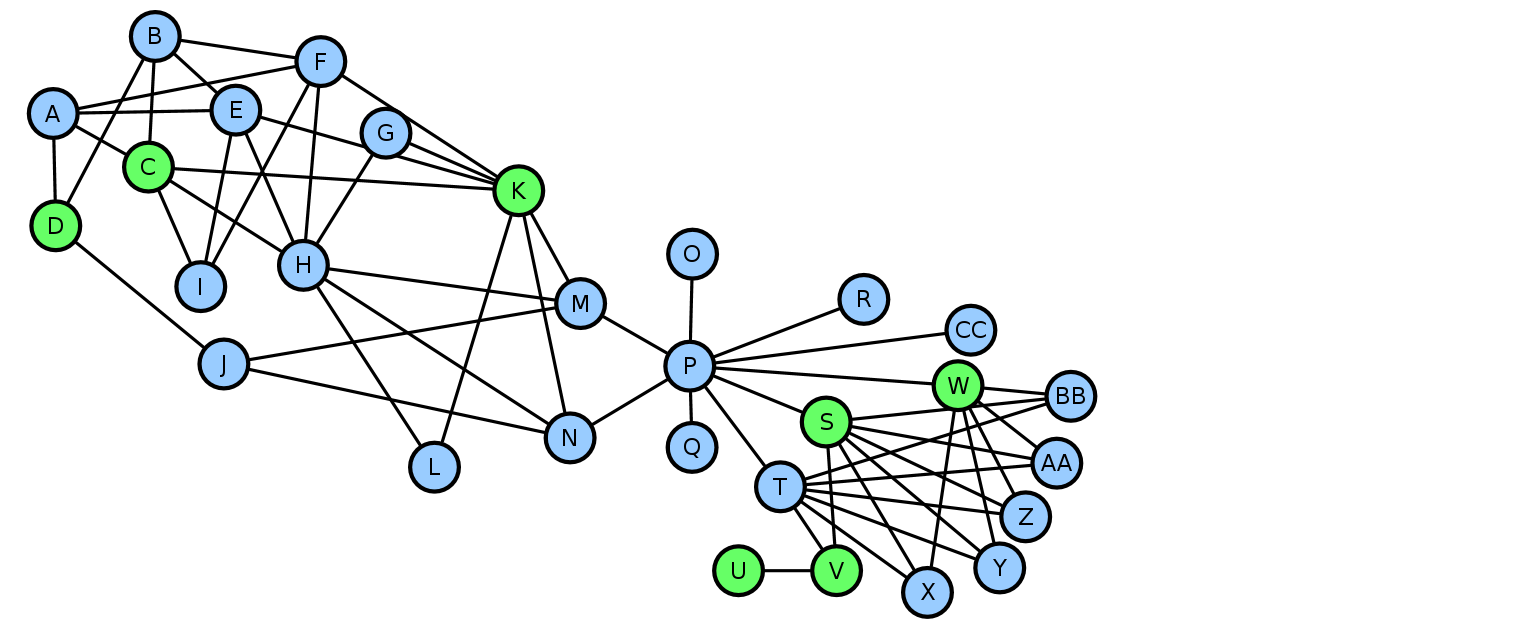
\includegraphics[width=10.0cm]{Tgfb1.png} 
		\caption{}
	\end{subfigure}
	\begin{subfigure}{.5\textwidth}
		\centering
		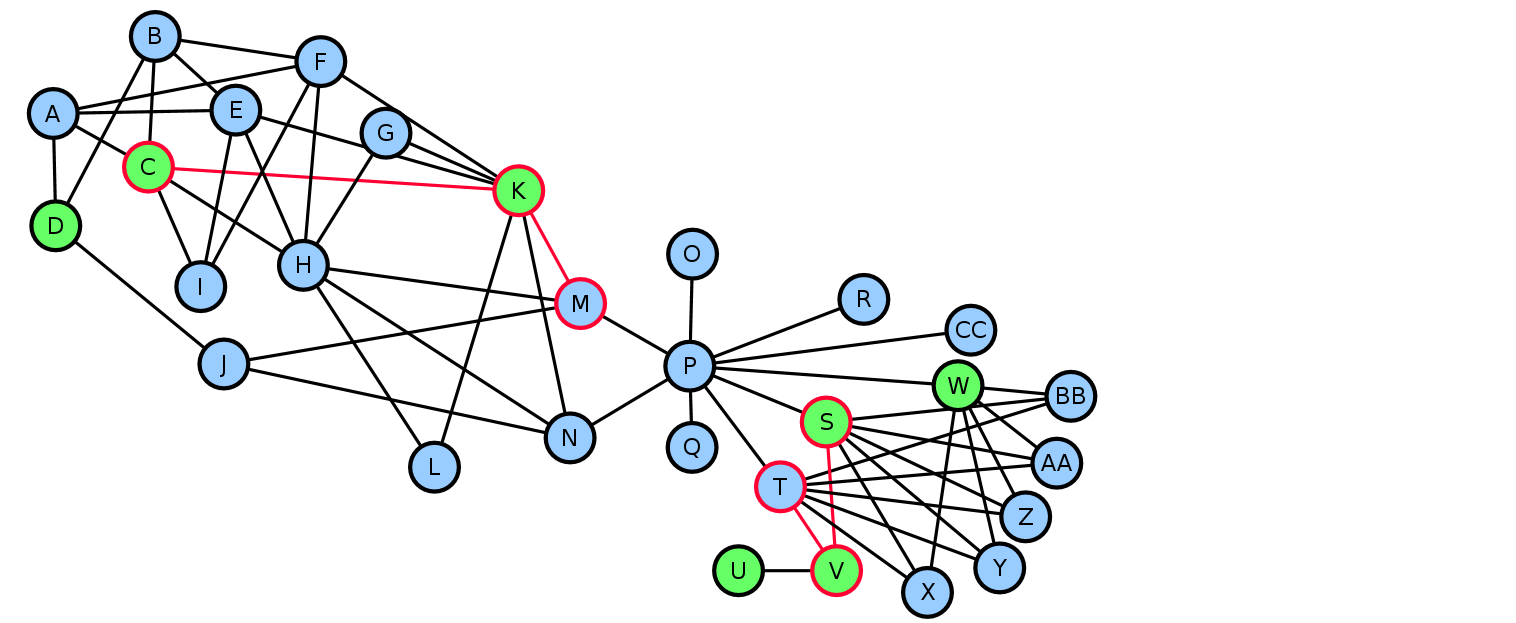
\includegraphics[width=10.0cm]{TGFBstep1.png}
		\caption{}
	\end{subfigure}
	\begin{subfigure}{.5\textwidth}
		\centering
		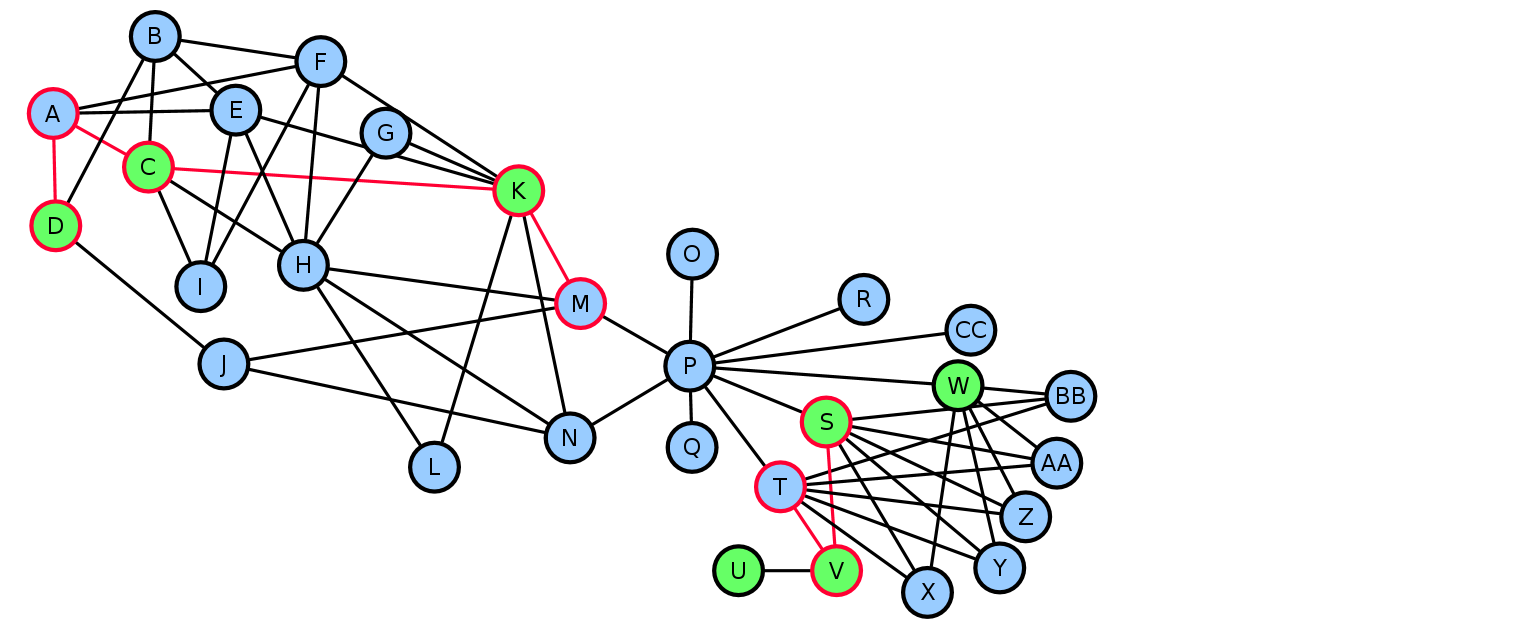
\includegraphics[width=10.0cm]{TGFBstep2.png} 
		\caption{}
	\end{subfigure}
	\begin{subfigure}{.5\textwidth}
		\centering
		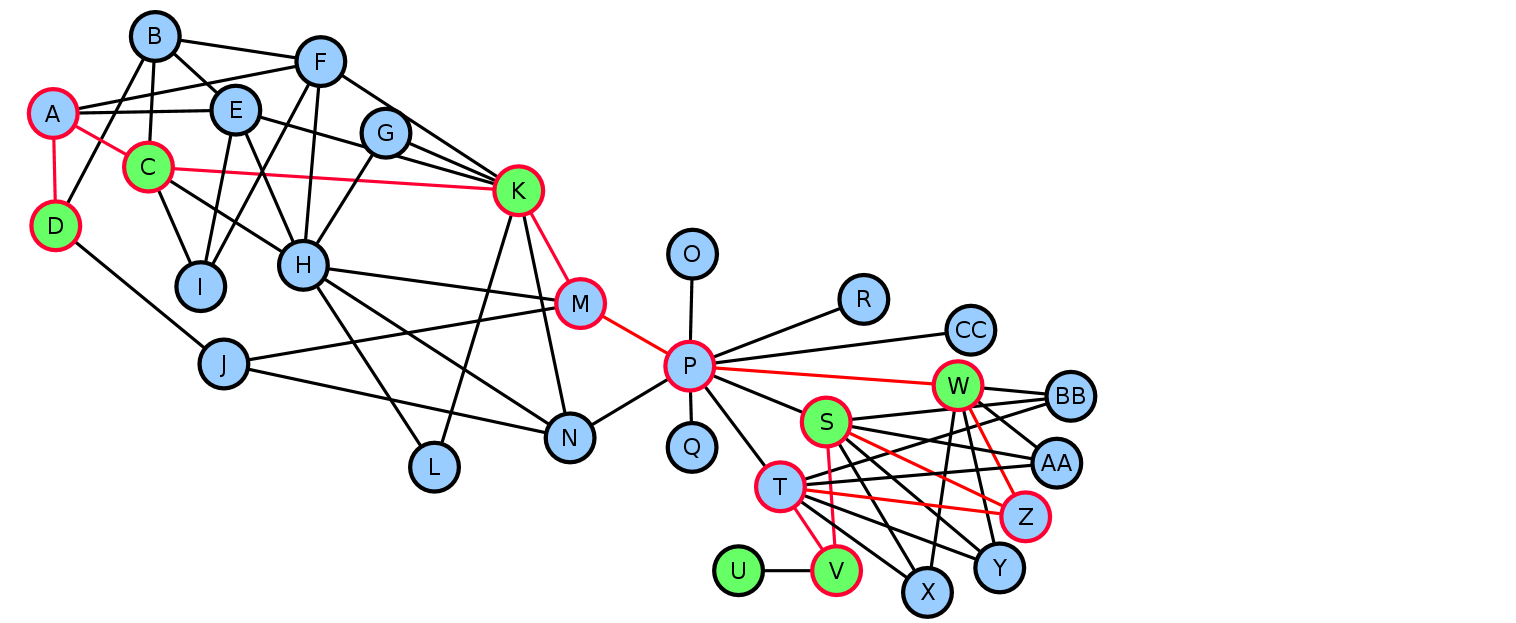
\includegraphics[width=10.0cm]{TGFBstep3.png}
		\caption{}
	\end{subfigure}
	\caption{Overview of \texttt{MSF} process showing the steps to identify the modulated sub-paths. (a) showing a network of genes with green nodes as genes with \textit{p}-values $< $ 0.05, and blue nodes are genes with \textit{p}-values $>$ 0.05, (b) the genes circled red show the two initial modulated sub-paths, sub-path1 found one with M,K,C and the second modulated sub-path2 S,V,T, (c) shows the modulated sub-path1 being extended to M,K,C,A,D, (d) shows both the modulated sub=paths merged with the addition of 3 genes Z,W,P.}
\end{figure*}

\begin{table*}[]
	\centering
	\caption{Comparison of gene enrichment analysis of MSF 6hpi sub-modules with SPIA pathway analysis}
	\label{Comparison of gene enrichment analysis of MSF 6hpi sub-modules with SPIA pathway analysis}
	\begin{tabular}{|l|l|}
		\hline
		\textbf{MSF Sub-module Gene Enrichment}              & \textbf{SPIA Pathway Analysis}            \\ \hline
		Toll-like receptor signaling pathway                 & Cytokine-cytokine receptor interaction    \\ \hline
		TNF signaling pathway                                & Chemokine signaling pathway               \\ \hline
		Prion diseases                                       & Apoptosis                                 \\ \hline
		Pertussis                                            & Taste transduction                        \\ \hline
		Type II diabetes mellitus                            & Influenza A                               \\ \hline
		Thyroid cancer                                       & NF-kappa B signaling pathway              \\ \hline
		Toxoplasmosis                                        & Type II diabetes mellitus                 \\ \hline
		Prolactin signaling pathway                          & Osteoclast differentiation                \\ \hline
		Cytosolic DNA-sensing pathway                        & Cytosolic DNA-sensing pathway             \\ \hline
		Chagas disease (American trypanosomiasis)            & Natural killer cell mediated cytotoxicity \\ \hline
		RIG-I-like receptor signaling pathway                & Measles                                   \\ \hline
		Th1 and Th2 cell differentiation                     & Amyotrophic lateral sclerosis (ALS)       \\ \hline
		Chemokine signaling pathway                          & Salivary secretion                        \\ \hline
		IL-17 signaling pathway                              & HTLV-I infection                          \\ \hline
		AGE-RAGE signaling pathway in diabetic complications & MAPK signaling pathway                    \\ \hline
		Measles                                              & Calcium signaling pathway                 \\ \hline
		Jak-STAT signaling pathway                           & Notch signaling pathway                   \\ \hline
		Leishmaniasis                                        & Graft-versus-host disease                 \\ \hline
		Endometrial cancer                                   & Maturity onset diabetes of the young      \\ \hline
		ECM-receptor interaction                             & Herpes simplex infection                  \\ \hline
		
		
		
	\end{tabular}
\end{table*}

\begin{table*}[]
	\centering
	\caption{Comparison of gene enrichment analysis of MSF 6hpi sub-modules with Reactome pathway enrichment analysis}
	\label{my-label}
	\begin{tabular}{|l|l|}
		\hline
		\textbf{MSF Sub-module Gene Enrichment}          & \textbf{Reactome Pathway Enrichment Analysis}   \\ \hline
		Signaling by Interleukins                        & Interferon alpha/beta signaling                 \\ \hline
		Interleukin-10 signaling                         & Interferon Signaling                            \\ \hline
		Cytokine Signaling in Immune system              & Interleukin-10 signaling                        \\ \hline
		Interleukin-6 family signaling                   & Cytokine Signaling in Immune system             \\ \hline
		Growth hormone receptor signaling                & Signaling by Interleukins                       \\ \hline
		Chemokine receptors bind chemokines              & Interferon gamma signaling                      \\ \hline
		Interleukin-4 and 13 signaling                   & Interleukin-4 and 13 signaling                  \\ \hline
		Signalling by NGF                                & Chemokine receptors bind chemokines             \\ \hline
		IL-6-type cytokine receptor ligand interactions  & RIG-I/MDA5 mediated induction of IFN-alpha/beta \\ \hline
		GPVI-mediated activation cascade                 & Negative regulators of RIG-I/MDA5 signaling     \\ \hline
		MyD88 dependent cascade initiated on endosome    & Nucleotide-binding domain                       \\ \hline
		Toll Like Receptor 7/8 (TLR7/8) Cascade          & NF-kB activation through FADD/RIP-1 pathway     \\ \hline
		Activated TLR4 signalling                        & Ovarian tumor domain proteases                  \\ \hline
		CD28 dependent PI3K/Akt signaling                & GPCR ligand binding                             \\ \hline
		Toll Like Receptor 9 (TLR9) Cascade              & Interleukin-1 processing                        \\ \hline
		CD28 co-stimulation                              & TRAF3-dependent IRF activation pathway          \\ \hline
		NGF signalling via TRKA from the plasma membrane & Interleukin-6 family signaling                  \\ \hline
		Toll Like Receptor 3 (TLR3) Cascade              & Class A/1 (Rhodopsin-like receptors)            \\ \hline
		TRIF-mediated TLR3/TLR4 signaling                & Inflammasomes                                   \\ \hline
		MyD88-independent TLR3/TLR4 cascade              & Interleukin-1 signaling                         \\ \hline
	\end{tabular}
\end{table*}

\begin{figure*}[th]
	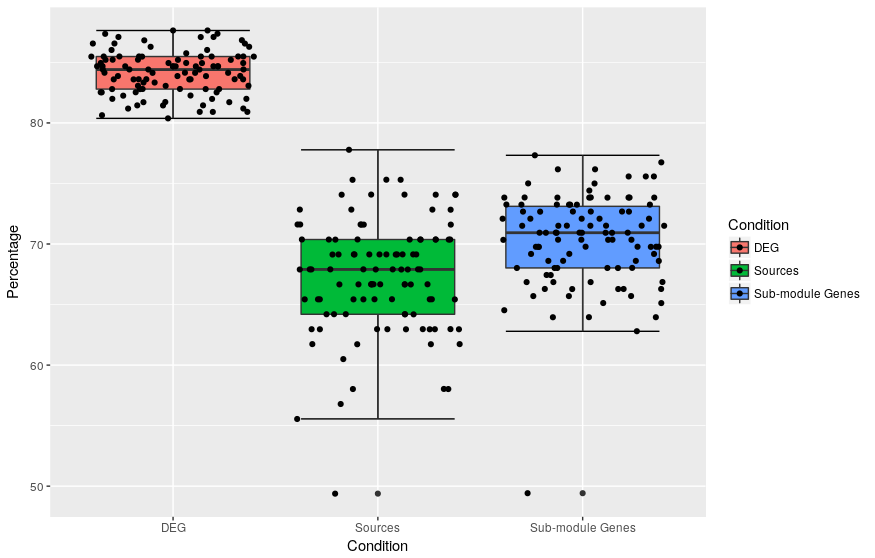
\includegraphics[width=16cm]{AllDEGSources}
	\caption{}
	\label{fig:alldegsources}
\end{figure*}

\begin{figure*}[p]
	\centering
	\includegraphics[width=14cm]{"SubPath Robustness 6H"}
\caption{}
\label{fig:subpath-robustness-6h}
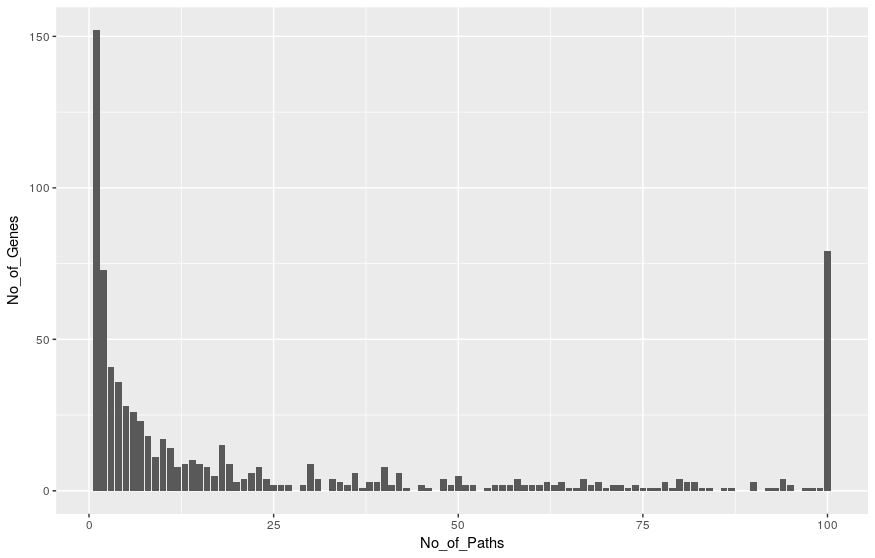
\includegraphics[width=14cm]{Betweeness}
\caption{}
\label{fig:betweeness}
\end{figure*}







\end{document}
